\begin{minipage}[t]{0.49\linewidth}
\centering
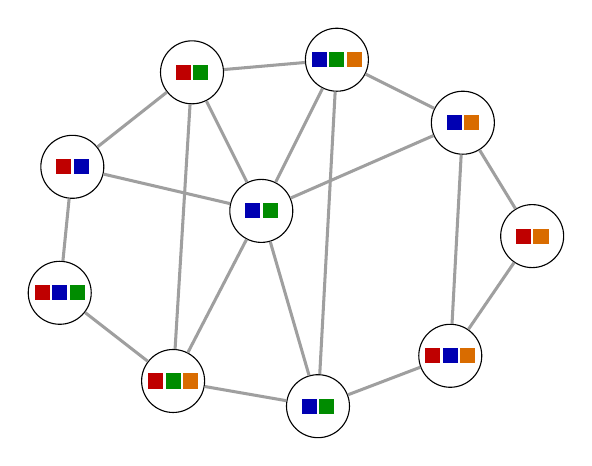
\begin{tikzpicture}[scale=0.80]
    \colorlet{iface1}{red!75!black}
    \colorlet{iface2}{blue!70!black}
    \colorlet{iface3}{green!55!black}
    \colorlet{iface4}{orange!85!black}

    % vertices
    \node[circle, draw, minimum size=8mm, inner sep=0pt] (v1) at (0.0,1.2) {};
    \node[circle, draw, minimum size=8mm, inner sep=0pt] (v2) at (1.9,2.7) {};
    \node[circle, draw, minimum size=8mm, inner sep=0pt] (v3) at (4.2,2.9) {};
    \node[circle, draw, minimum size=8mm, inner sep=0pt] (v4) at (6.2,1.9) {};
    \node[circle, draw, minimum size=8mm, inner sep=0pt] (v5) at (7.3,0.1) {};
    \node[circle, draw, minimum size=8mm, inner sep=0pt] (v6) at (6.0,-1.8) {};
    \node[circle, draw, minimum size=8mm, inner sep=0pt] (v7) at (3.9,-2.6) {};
    \node[circle, draw, minimum size=8mm, inner sep=0pt] (v8) at (1.6,-2.2) {};
    \node[circle, draw, minimum size=8mm, inner sep=0pt] (v9) at (-0.2,-0.8) {};
    \node[circle, draw, minimum size=8mm, inner sep=0pt] (v10) at (3.0,0.5) {};

    % edges
    \draw[gray!75, line width=1.1pt] (v1) -- (v2) -- (v3) -- (v4) -- (v5) -- (v6) -- (v7) -- (v8) -- (v9) -- (v1);
    \draw[gray!75, line width=1.1pt] (v1) -- (v10);
    \draw[gray!75, line width=1.1pt] (v2) -- (v10);
    \draw[gray!75, line width=1.1pt] (v3) -- (v10);
    \draw[gray!75, line width=1.1pt] (v4) -- (v10);
    \draw[gray!75, line width=1.1pt] (v7) -- (v10);
    \draw[gray!75, line width=1.1pt] (v8) -- (v10);
    \draw[gray!75, line width=1.1pt] (v2) -- (v8);
    \draw[gray!75, line width=1.1pt] (v3) -- (v7);
    \draw[gray!75, line width=1.1pt] (v4) -- (v6);

    % available label rectangles in nodes
    \begin{scope}[shift={(v1.center)}]
        \fill[iface1] (-0.26,-0.12) rectangle (-0.02,0.12);
        \fill[iface2] (0.02,-0.12) rectangle (0.26,0.12);
    \end{scope}
    \begin{scope}[shift={(v2.center)}]
        \fill[iface1] (-0.26,-0.12) rectangle (-0.02,0.12);
        \fill[iface3] (0.02,-0.12) rectangle (0.26,0.12);
    \end{scope}
    \begin{scope}[shift={(v3.center)}]
        \fill[iface2] (-0.40,-0.12) rectangle (-0.16,0.12);
        \fill[iface3] (-0.12,-0.12) rectangle (0.12,0.12);
        \fill[iface4] (0.16,-0.12) rectangle (0.40,0.12);
    \end{scope}
    \begin{scope}[shift={(v4.center)}]
        \fill[iface2] (-0.26,-0.12) rectangle (-0.02,0.12);
        \fill[iface4] (0.02,-0.12) rectangle (0.26,0.12);
    \end{scope}
    \begin{scope}[shift={(v5.center)}]
        \fill[iface1] (-0.26,-0.12) rectangle (-0.02,0.12);
        \fill[iface4] (0.02,-0.12) rectangle (0.26,0.12);
    \end{scope}
    \begin{scope}[shift={(v6.center)}]
        \fill[iface1] (-0.40,-0.12) rectangle (-0.16,0.12);
        \fill[iface2] (-0.12,-0.12) rectangle (0.12,0.12);
        \fill[iface4] (0.16,-0.12) rectangle (0.40,0.12);
    \end{scope}
    \begin{scope}[shift={(v7.center)}]
        \fill[iface2] (-0.26,-0.12) rectangle (-0.02,0.12);
        \fill[iface3] (0.02,-0.12) rectangle (0.26,0.12);
    \end{scope}
    \begin{scope}[shift={(v8.center)}]
        \fill[iface1] (-0.40,-0.12) rectangle (-0.16,0.12);
        \fill[iface3] (-0.12,-0.12) rectangle (0.12,0.12);
        \fill[iface4] (0.16,-0.12) rectangle (0.40,0.12);
    \end{scope}
    \begin{scope}[shift={(v9.center)}]
        \fill[iface1] (-0.40,-0.12) rectangle (-0.16,0.12);
        \fill[iface2] (-0.12,-0.12) rectangle (0.12,0.12);
        \fill[iface3] (0.16,-0.12) rectangle (0.40,0.12);
    \end{scope}
    \begin{scope}[shift={(v10.center)}]
        \fill[iface2] (-0.26,-0.12) rectangle (-0.02,0.12);
        \fill[iface3] (0.02,-0.12) rectangle (0.26,0.12);
    \end{scope}
\end{tikzpicture}

\vspace{1mm}
{\scriptsize Available labels}
\end{minipage}
\hfill
\begin{minipage}[t]{0.49\linewidth}
\centering
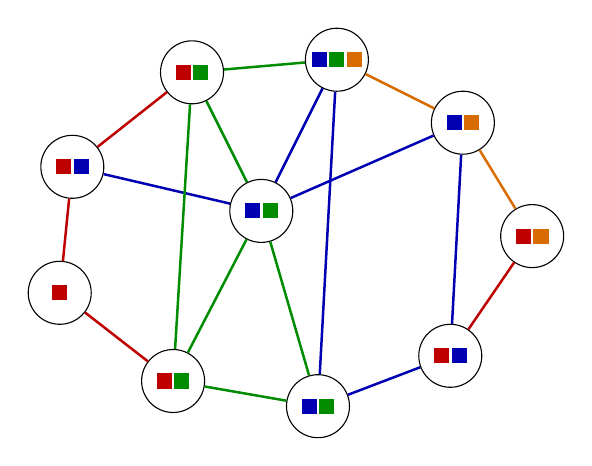
\begin{tikzpicture}[scale=0.80]
    \colorlet{iface1}{red!75!black}
    \colorlet{iface2}{blue!70!black}
    \colorlet{iface3}{green!55!black}
    \colorlet{iface4}{orange!85!black}

    % vertices
    \node[circle, draw, minimum size=8mm, inner sep=0pt] (v1) at (0.0,1.2) {};
    \node[circle, draw, minimum size=8mm, inner sep=0pt] (v2) at (1.9,2.7) {};
    \node[circle, draw, minimum size=8mm, inner sep=0pt] (v3) at (4.2,2.9) {};
    \node[circle, draw, minimum size=8mm, inner sep=0pt] (v4) at (6.2,1.9) {};
    \node[circle, draw, minimum size=8mm, inner sep=0pt] (v5) at (7.3,0.1) {};
    \node[circle, draw, minimum size=8mm, inner sep=0pt] (v6) at (6.0,-1.8) {};
    \node[circle, draw, minimum size=8mm, inner sep=0pt] (v7) at (3.9,-2.6) {};
    \node[circle, draw, minimum size=8mm, inner sep=0pt] (v8) at (1.6,-2.2) {};
    \node[circle, draw, minimum size=8mm, inner sep=0pt] (v9) at (-0.2,-0.8) {};
    \node[circle, draw, minimum size=8mm, inner sep=0pt] (v10) at (3.0,0.5) {};

    % edges colored by covering label
    \draw[iface1, line width=0.9pt] (v1) -- (v2);
    \draw[iface3, line width=0.9pt] (v2) -- (v3);
    \draw[iface4, line width=0.9pt] (v3) -- (v4);
    \draw[iface4, line width=0.9pt] (v4) -- (v5);
    \draw[iface1, line width=0.9pt] (v5) -- (v6);
    \draw[iface2, line width=0.9pt] (v6) -- (v7);
    \draw[iface3, line width=0.9pt] (v7) -- (v8);
    \draw[iface1, line width=0.9pt] (v8) -- (v9);
    \draw[iface1, line width=0.9pt] (v9) -- (v1);
    \draw[iface2, line width=0.9pt] (v1) -- (v10);
    \draw[iface3, line width=0.9pt] (v2) -- (v10);
    \draw[iface2, line width=0.9pt] (v3) -- (v10);
    \draw[iface2, line width=0.9pt] (v4) -- (v10);
    \draw[iface3, line width=0.9pt] (v7) -- (v10);
    \draw[iface3, line width=0.9pt] (v8) -- (v10);
    \draw[iface3, line width=0.9pt] (v2) -- (v8);
    \draw[iface2, line width=0.9pt] (v3) -- (v7);
    \draw[iface2, line width=0.9pt] (v4) -- (v6);

    % selected labels in solution
    \begin{scope}[shift={(v1.center)}]
        \fill[iface1] (-0.26,-0.12) rectangle (-0.02,0.12);
        \fill[iface2] (0.02,-0.12) rectangle (0.26,0.12);
    \end{scope}
    \begin{scope}[shift={(v2.center)}]
        \fill[iface1] (-0.26,-0.12) rectangle (-0.02,0.12);
        \fill[iface3] (0.02,-0.12) rectangle (0.26,0.12);
    \end{scope}
    \begin{scope}[shift={(v3.center)}]
        \fill[iface2] (-0.40,-0.12) rectangle (-0.16,0.12);
        \fill[iface3] (-0.12,-0.12) rectangle (0.12,0.12);
        \fill[iface4] (0.16,-0.12) rectangle (0.40,0.12);
    \end{scope}
    \begin{scope}[shift={(v4.center)}]
        \fill[iface2] (-0.26,-0.12) rectangle (-0.02,0.12);
        \fill[iface4] (0.02,-0.12) rectangle (0.26,0.12);
    \end{scope}
    \begin{scope}[shift={(v5.center)}]
        \fill[iface1] (-0.26,-0.12) rectangle (-0.02,0.12);
        \fill[iface4] (0.02,-0.12) rectangle (0.26,0.12);
    \end{scope}
    \begin{scope}[shift={(v6.center)}]
        \fill[iface1] (-0.26,-0.12) rectangle (-0.02,0.12);
        \fill[iface2] (0.02,-0.12) rectangle (0.26,0.12);
    \end{scope}
    \begin{scope}[shift={(v7.center)}]
        \fill[iface2] (-0.26,-0.12) rectangle (-0.02,0.12);
        \fill[iface3] (0.02,-0.12) rectangle (0.26,0.12);
    \end{scope}
    \begin{scope}[shift={(v8.center)}]
        \fill[iface1] (-0.26,-0.12) rectangle (-0.02,0.12);
        \fill[iface3] (0.02,-0.12) rectangle (0.26,0.12);
    \end{scope}
    \begin{scope}[shift={(v9.center)}]
        \fill[iface1] (-0.12,-0.12) rectangle (0.12,0.12);
    \end{scope}
    \begin{scope}[shift={(v10.center)}]
        \fill[iface2] (-0.26,-0.12) rectangle (-0.02,0.12);
        \fill[iface3] (0.02,-0.12) rectangle (0.26,0.12);
    \end{scope}
\end{tikzpicture}

\vspace{1mm}
{\scriptsize Example covering assignment}
\end{minipage}
